
\documentclass[12pt]{report}
\usepackage{geometry}
\usepackage{url,enumerate, amssymb, multirow, anysize, booktabs, threeparttable, amsfonts, bbm}
\usepackage[colorlinks = true,
            linkcolor = blue,
            urlcolor  = blue,
            citecolor = blue,
            anchorcolor = blue]{hyperref}
\usepackage{setspace,listings,dsfont}
%\usepackage{cite}
\usepackage[square,numbers]{natbib}
\bibliographystyle{abbrvnat, lipsum}
\usepackage{mathrsfs, wrapfig}
\usepackage{hanging}
\renewcommand*\thesection{\arabic{section}}
\usepackage{color,soul,amssymb}
\usepackage{fancyhdr, mathtools}
\usepackage{dcolumn, capt-of}
\usepackage{indentfirst, verbatim}
\newcounter{equationset, sectsty, breqn}
\usepackage{setspace,float,lscape,subfigure,amsmath,multirow,color,nag}
\usepackage[font=sf, labelfont={sf,bf}, margin=1cm]{caption}
\captionsetup{font={small,sf,singlespacing}}
\newcommand{\pb}{\mathbb{P}}
\newcommand{\E}{\ensuremath{\mbox{E}}}
% Page style definition
\geometry{margin=1.0in}
\pagestyle{fancy}
% Customize this to your liking.
\setlength{\headheight}{16pt}
\lhead{}\chead{}\rhead{C. elegans Neuronal Network}\lfoot{}
\cfoot{\thepage}\rfoot{April, 2016}

\makeatletter
\def\@makechapterhead#1{%
  \vspace*{0\p@}%
  {\parindent \z@ \raggedright \normalfont
    \interlinepenalty\@M
    \Huge\bfseries  \thechapter.\quad #1\par\nobreak
    \vskip 25\p@
  }}
\makeatother


\usepackage{Sweave}
\begin{document}
\Sconcordance{concordance:report1.tex:report1.Rnw:%
1 45 1 1 0 338 1}



\pagenumbering{roman}


\pagenumbering{arabic}

\doublespace


\chapter{Testing Network Dependence Using Multiscale Graph Correlation} 
\normalsize


There have been a work on the properties of the neuronal network based on these incomplete or inconsistent wiring diagrams. Varshney et al(2011) proposed ``near-complete" wiring diagram of C. elegans. They are interested in local network properties as well as global network properties. We can naturally think that neuronal physical networks and some of the biological function or properties would be correlated each other.

We are given a connected, weighted and also directed network of C. elegans, which is comprised of 279 nodes and 3225 (directed) edges between them. The given network illustrates the network in the region of pharynx, and the weight imposed on each edge is equivalent to the number of corresponding synapses. For vertex attributes, we have (1) cell class, (2) soma position, (3) neurotransmitters and (4) role. To avoid the difficulties due to missingness, we are going to look into the complete data first - (1) cell class and (2) soma position.  

\section{Choosing distance matrix for network(graph)}

\textit{Most of the works are borrowed from Minh Tang's thesis ``Graph metrics and dimension reduction"}

First we have considered a few candidiates for distances on graphs. The first one is a dissimilarity matrix $A$ where $A_{ij} = 1$ if node $i$ and node $j$ are not adjacent or their is no edge starting from $i$ to $j$. The second candidate distance measure is a geodesic distance, which is defined as the shortest path length of consecutive edges connecting two nodes. Dissimilarity matrix is a part of geodesic distance. We have observed that these two measures are two extremes of opposite side. Maybe we want more than adjacency relationship and using all the path information, i.e. geodesic distance, may be too much. We assume that \textit{Diffusion distances} may provide a distnaces somewhere between the two. 



\subsection{Distances on undirected graphs}

- Similarity measure $\omega$

$$\omega[i,j] = \mbox{ (the number of synapses starting from i to j)}$$
 

- Transition probability (Assume time homogeneous Markov chain; left stochastic matrix)

$$P[i,j] = Pr\big( X_{n} = j  | X_{n-1} = i \big)$$

We define the transition matrix \textbf{P} = $(p_{ij})$ of a Markov chain as:

$$p_{ij} = \left\{ \begin{array}{ll} \frac{w(\{ i, j\})}{ deg(i) } & \mbox{ if } u \sim v \\ 0 & \mbox{ otherwise }  \end{array}  \right.$$


\begin{figure}[H]
\captionsetup{format=plain}
\centering
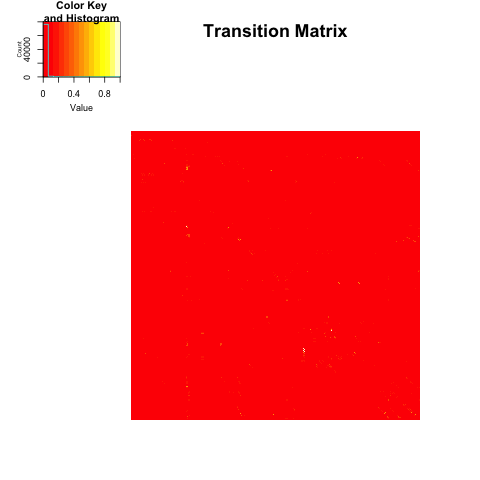
\includegraphics[width=0.4\textwidth]{../figure/trans.png}
\caption{Transition matrix P}
\label{fig:trans}
\end{figure}




- Stationary distribution 
: A probability vector $\pi$ is a stationary distribution for Markov chain $P$ if $\pi P = \pi$. Over the long run, no matter what the starting state was, the proportion of time the chain spends in node $j$ is approximately $\pi(j) (j = 1, ... , n)$.
Use \verb!statdistr! in r.

\begin{figure}[H]
\captionsetup{format=plain}
\centering
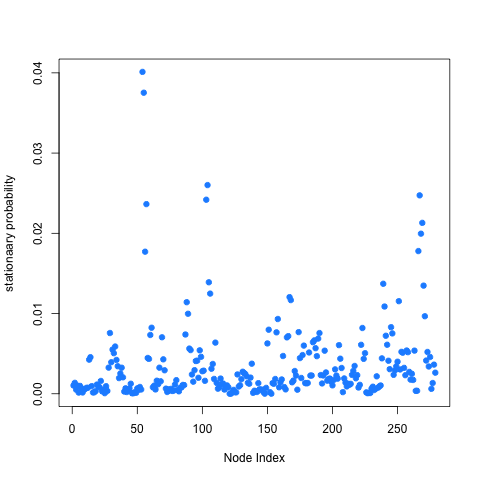
\includegraphics[width=0.4\textwidth]{../figure/statd.png}
\caption{Stationary probability based on P}
\label{fig:statd}
\end{figure}



  Let $G = (V, E, \omega)$ be an undirected graph with $\omega$ being a similarity measure between vertices of $V.$ Denote by $\textbf{P}$ the probability transition matrix of $G.$ The diffusion distance at time $t,$ $\rho_{t}(u,v)$, between two nodes $u,v \in V$ is defined as:
  
  $$\rho^2_{t} = \sum\limits_{w \in V}\big( \textbf{P}^{t}(u,w) - \textbf{P}^{t}(v,w) \big)^2 \frac{1}{\pi(w)} =  \kappa(\textbf{P}^{2t} \Pi^{-1} )$$

 
Diffusion distances for Directed Graph at time $t$ is defined as :

$$\Delta_{\rho^{2}_{t}} = \kappa(\textbf{P}^{t} \Pi^{-1} (\textbf{P}^{t})^{T} )$$
 
where $\kappa(\textbf{A}) = \textbf{A}_{dg} \textbf{1} \textbf{1}^{T} - \textbf{A} - \textbf{A}^{T} + \textbf{1} \textbf{1}^{T} \textbf{A}_{dg}$ 
 
 
\begin{figure}[H]
\captionsetup{format=plain}
\centering
\subfigure[dissimilarity matrix]{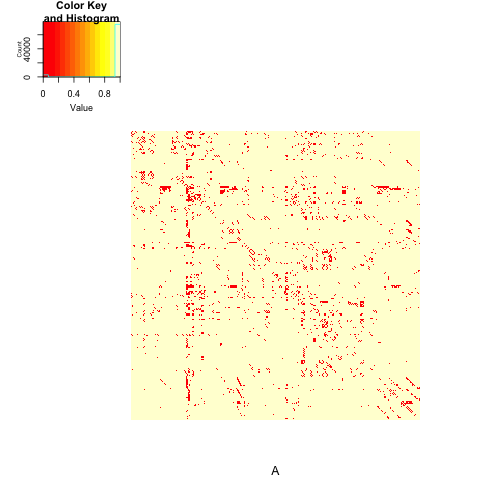
\includegraphics[width=0.3\textwidth]{../figure/A_plot.png}}
\subfigure[t=1]{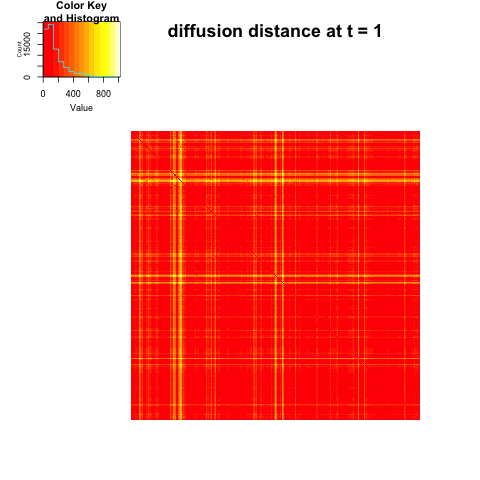
\includegraphics[width=0.3\textwidth]{../figure/diffusion1}}
\subfigure[t=5]{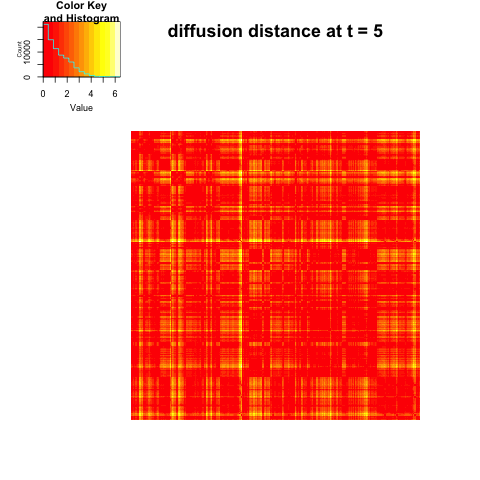
\includegraphics[width=0.3\textwidth]{../figure/diffusion5.png}}
\caption{Heatmap of distance measures}
\label{fig:dist}    
\end{figure} 
 
 
 
\begin{figure}[H]
\captionsetup{format=plain}
\centering
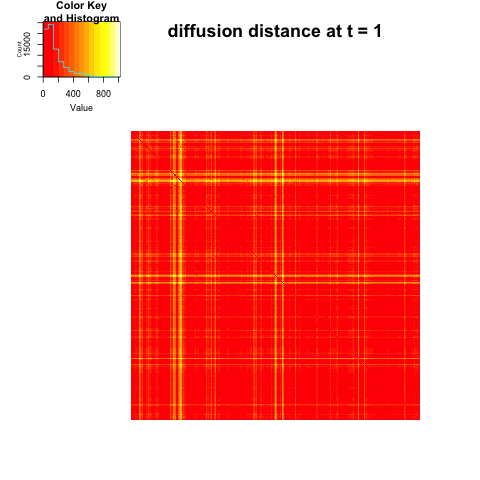
\includegraphics[width=0.4\textwidth]{../figure/diffusion1.png}
\caption{Diffusion distances of neuronal network at time t = 1}
\label{fig:statd}
\end{figure} 
 
 
- Difficulties of applying diffusion distance to categorical variable graph : $G$ must be connected. Otherwise, transition probability between different categories will be zero.  
 
 \section{Neuronal Network vs. Soma position}
 
 Soma position, among those four attributes, is the only attribute that can be treated as a continuous variable.
 - $\textbf{A}$ :  Distance matrix based on an adjacency matrix of $A$ for which $A_{ij} = 0$ if and only if there exists an edge from node $i$ to node $j$; $A_{ij} = 1$ if they are NOT adjacent each other. 

- \textbf{$A^\prime$} Geodesic distance matrix $A$ weighted by the count of synapses, using Dijkstra algorithm.
  
- $\textbf{B}$ : $B_{ij} = (1 - \exp(-|X_{i} - X_{j}|)) / \max(B_{ij} ; i,j = 1,...,n)$

- \textbf{$B^\prime$} : Euclidean distance matrix of soma position.

- $\tilde{A} = H A H$ for any matrix $A$



\begin{center}\textbf{Goal : Test $H_{0} : f_{AB} = f_{A}f_{B}$}
\end{center} 
 
\begin{figure}[H]
\captionsetup{format=plain}
\centering
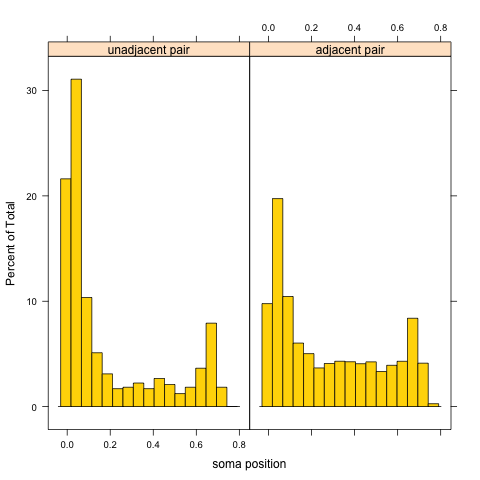
\includegraphics[width=0.4\textwidth]{../figure/histo1.png}
\caption{distribution of soma position unadjacent pairs vs. adjacent pairs}
\label{fig:histo1}
\end{figure}  
 
 
\begin{figure}[H]
\captionsetup{format=plain}
\centering
\subfigure[A]{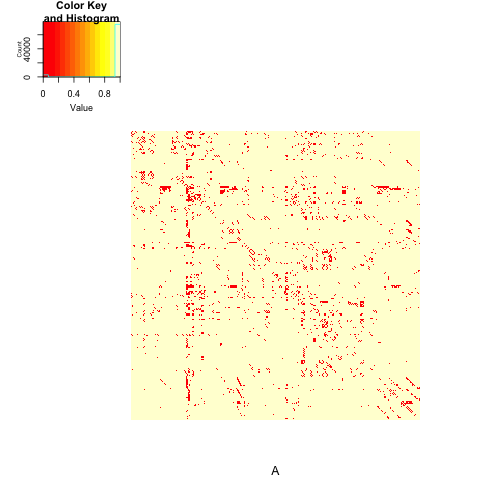
\includegraphics[width=0.3\textwidth]{../figure/A_plot.png}}
\subfigure[B]{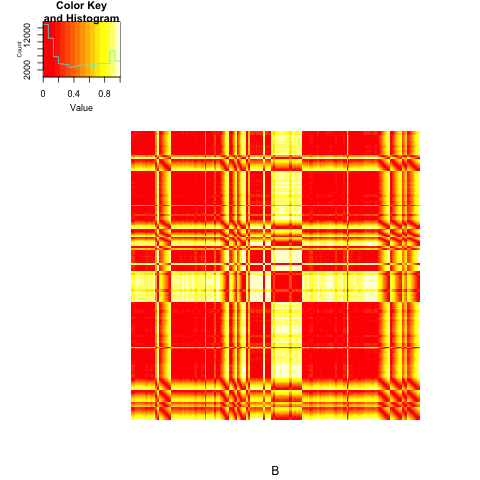
\includegraphics[width=0.3\textwidth]{../figure/B_plot.png}}
\subfigure[A $\cdot$ B]{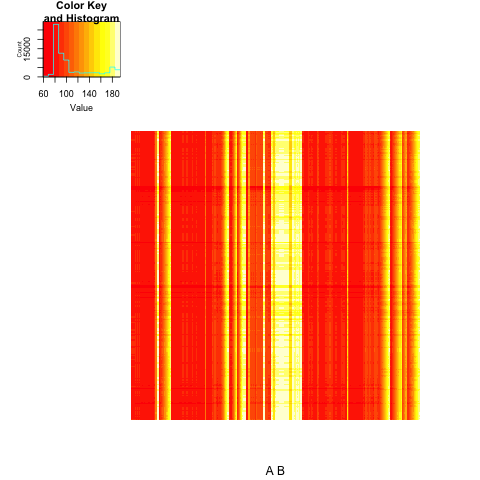
\includegraphics[width=0.3\textwidth]{../figure/AB_plot.png}}
\subfigure[$\tilde{A}$]{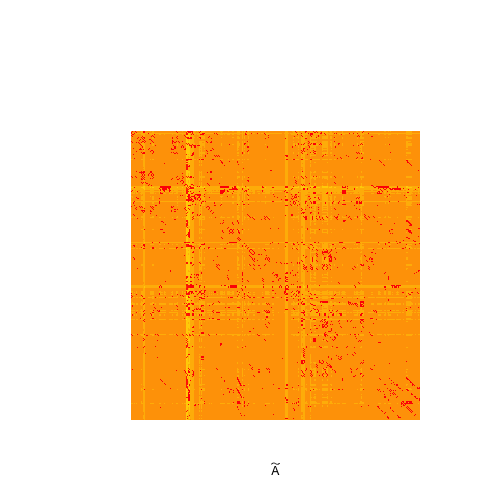
\includegraphics[width=0.3\textwidth]{../figure/HAH.png}}
\subfigure[$\tilde{B}$]{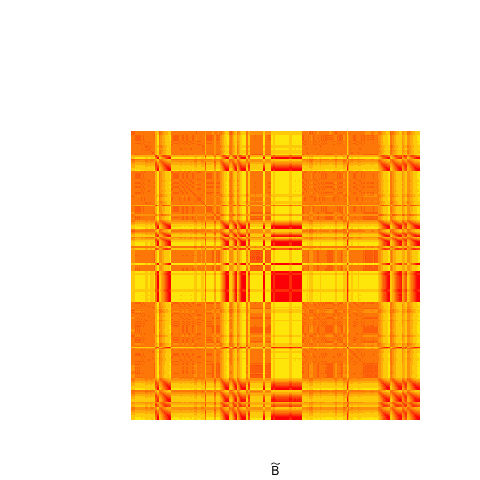
\includegraphics[width=0.3\textwidth]{../figure/HBH.png}}
\subfigure[$\widetilde{A \cdot B}$]{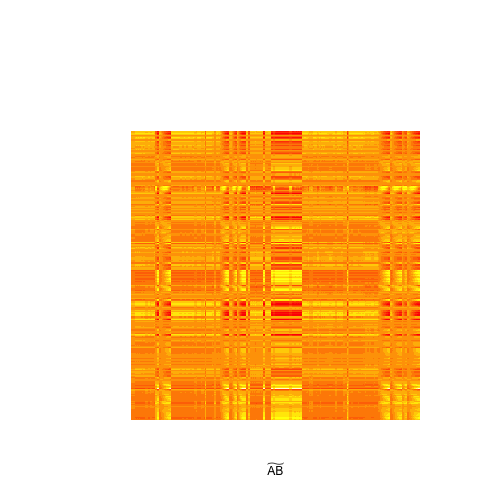
\includegraphics[width=0.3\textwidth]{../figure/HABH.png}}
\caption{Heatmap of dissimilarity measures}
\label{fig:subnetwork}    
\end{figure}


\begin{figure}[H]
\captionsetup{format=plain}
\centering
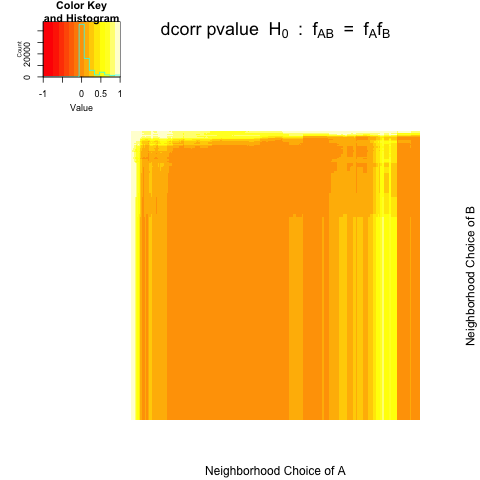
\includegraphics[width=0.4\textwidth]{../figure/P_A_B.png}
\caption{Local p-value matrix A vs B}
\label{fig:PAB}
\end{figure}


\begin{figure}[H]
\captionsetup{format=plain}
\centering
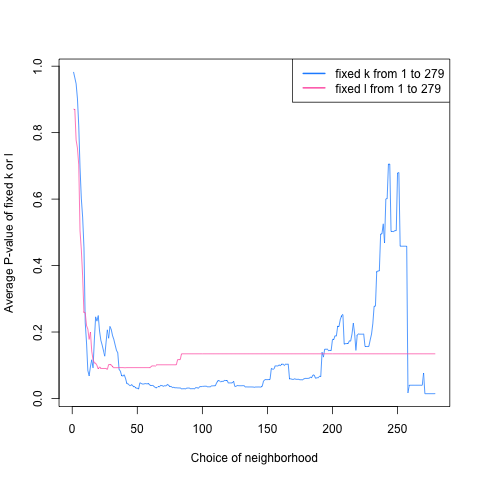
\includegraphics[width=0.4\textwidth]{../figure/AB_hist.png}
\caption{Local p-value depending on choice of neighborhood}
\label{fig:ABhist}
\end{figure}


%%%%%%%%%%%%%%%%%%%%%%%%%%%%%%%%%%%%%%%%%%%%%%%%%%%%%%%%%%%%%%%%%%%%%
\newpage
\begin{center}\textbf{Goal : Test $H_{0} : f_{A^\prime B^\prime} = f_{A^\prime}f_{B^\prime}$}
\end{center} 

\begin{figure}[H]
\captionsetup{format=plain}
\centering
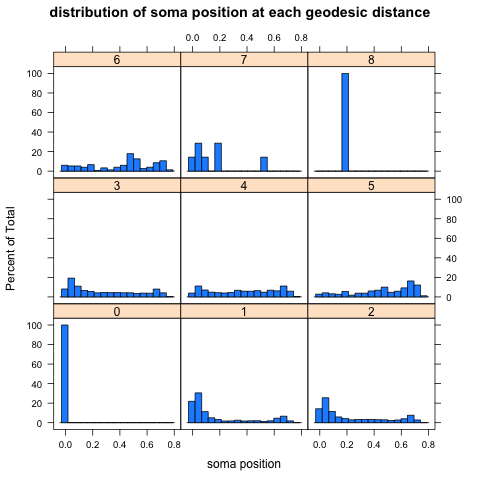
\includegraphics[width=0.4\textwidth]{../figure/histo2.png}
\caption{distribution of soma position across geodesic distance}
\label{fig:histo1}
\end{figure}  
 



\begin{figure}[H]
\captionsetup{format=plain}
\subfigure[$A^\prime$]{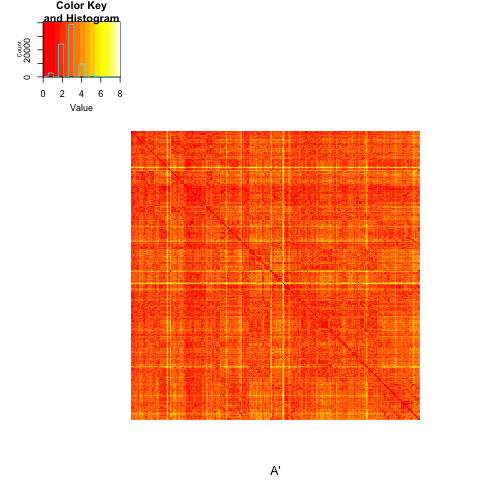
\includegraphics[width=0.3\textwidth]{../figure/A2_plot.png}}
\subfigure[$B^\prime$]{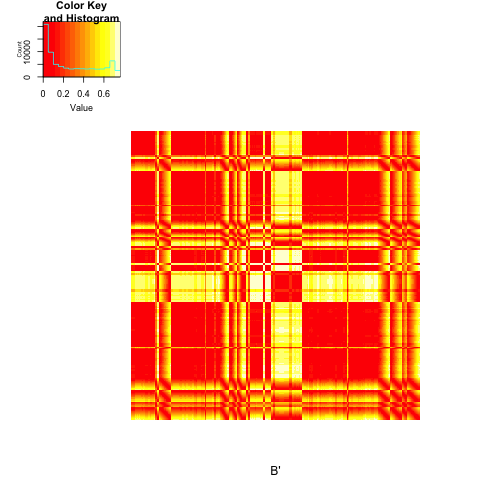
\includegraphics[width=0.3\textwidth]{../figure/B2_plot.png}}
\subfigure[$A^\prime B^\prime$]{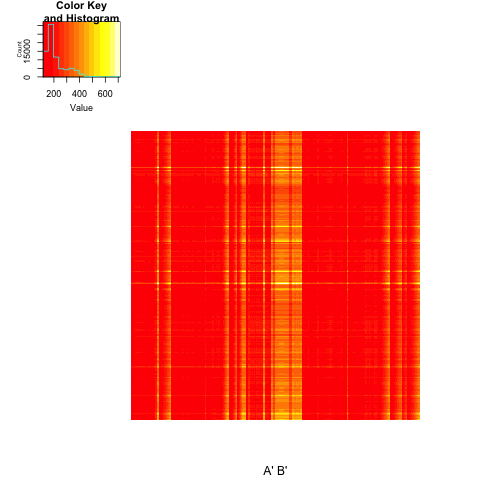
\includegraphics[width=0.3\textwidth]{../figure/A2B2_plot.png}}
\subfigure[$\widetilde{A^\prime}$]{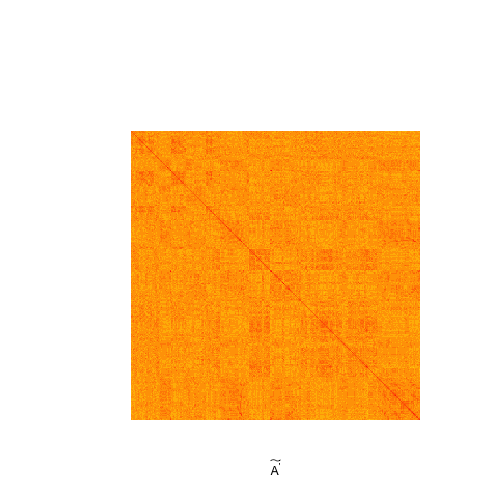
\includegraphics[width=0.3\textwidth]{../figure/HA2H.png}}
\subfigure[$\widetilde{B^\prime}$]{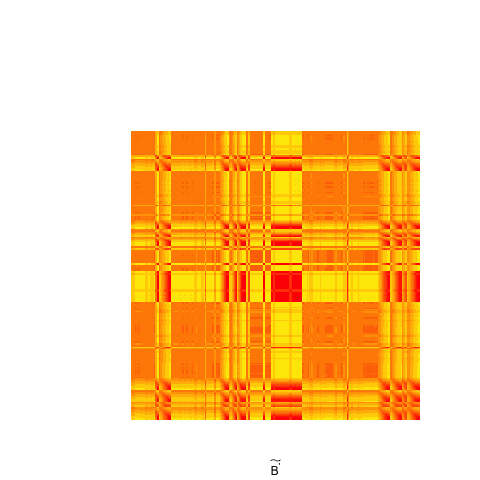
\includegraphics[width=0.3\textwidth]{../figure/HB2H.png}}
\subfigure[$\widetilde{A^\prime B^\prime}$]{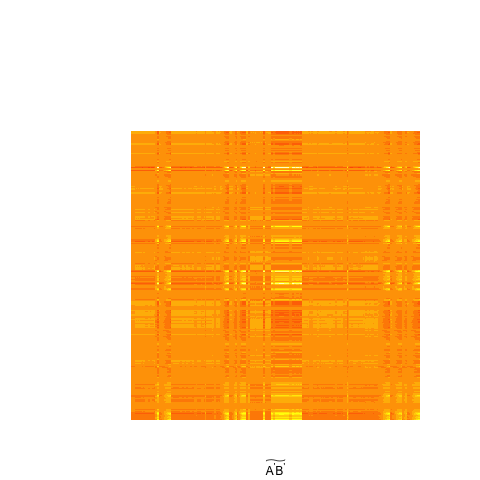
\includegraphics[width=0.3\textwidth]{../figure/HA2B2H.png}}
\caption{Heatmap of Geodesic Distance $\& $Euclidean Distance}
\label{fig:table}    
\end{figure}


\begin{figure}[H]
\captionsetup{format=plain}
\centering
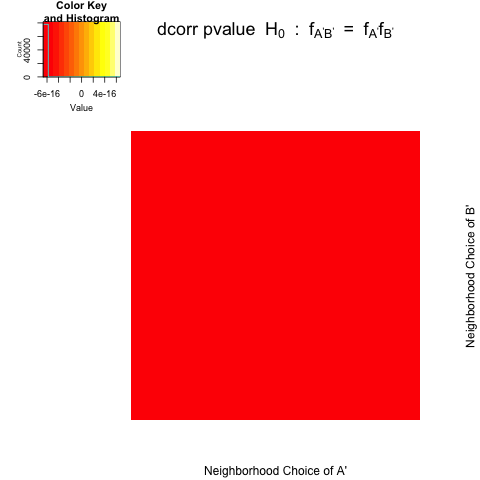
\includegraphics[width=0.4\textwidth]{../figure/P_A2_E.png}
\caption{Local p-value matrix $A^\prime$ vs $B^\prime$}
\label{fig:PA2E}
\end{figure} 


P-values, in overall, shows lower value, or lowest value in the second hypothesis. (Euclidean distance measure is more sensitive than dissimilarity measure)

%%%%%%%%%%%%%%%%%%%%%%%%%%%%%%%%%%%%%%%%%%%%%%%%%%%%%%%%%%%%%%%%%%%%
\newpage
\section{Neuronal Network vs. Cell type}
 
 
- \textbf{C} : Dissimilarity matrix of Cell type $\&$ Cell Direction categories. - Right(96), Left(93), and other 24 categories(90).  
 
\begin{center}\textbf{Goal : Test $H_{0} : f_{AC} = f_{A}f_{C}$}
\end{center}  
 
 
\begin{figure}[H]
\captionsetup{format=plain}
\subfigure[$A$]{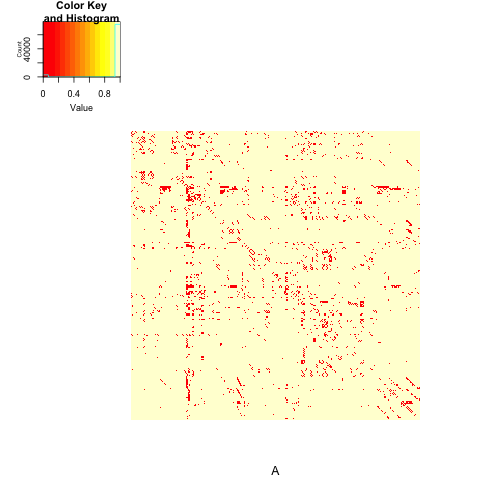
\includegraphics[width=0.3\textwidth]{../figure/A_plot.png}}
\subfigure[$C$]{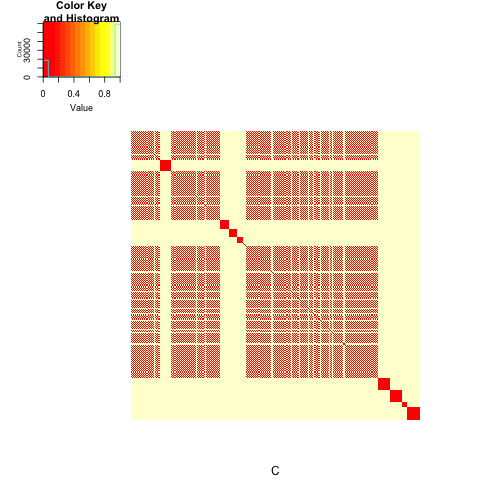
\includegraphics[width=0.3\textwidth]{../figure/C_plot.png}}
\subfigure[$A \cdot C$]{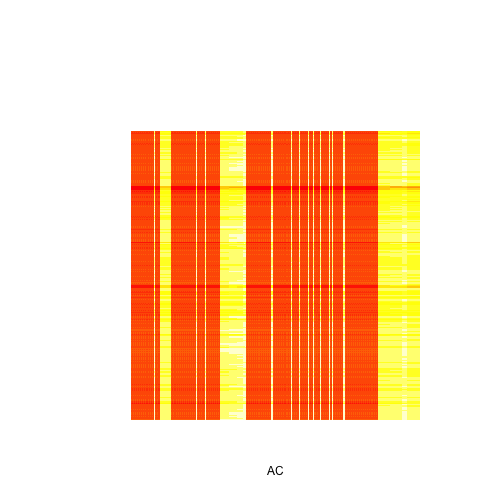
\includegraphics[width=0.3\textwidth]{../figure/AC_plot.png}}
\end{figure}

\begin{figure}[H]
\captionsetup{format=plain}
\subfigure[$\widetilde{A}$]{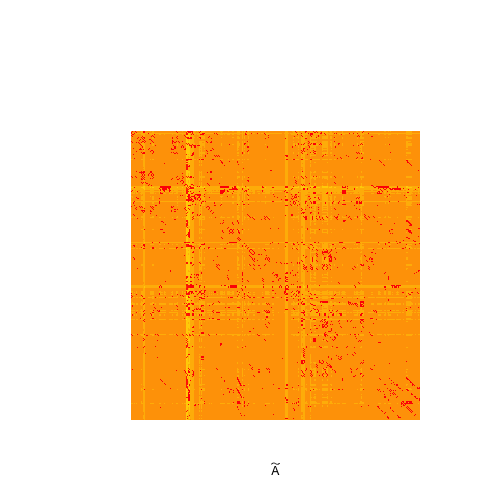
\includegraphics[width=0.3\textwidth]{../figure/HAH.png}}
\subfigure[$\widetilde{C}$]{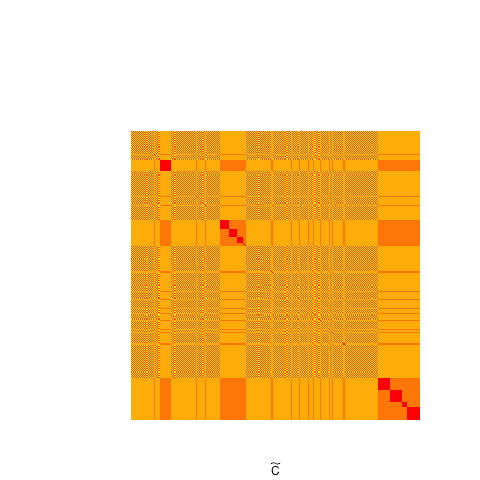
\includegraphics[width=0.3\textwidth]{../figure/HCH_plot.png}}
\subfigure[$\widetilde{A C}$]{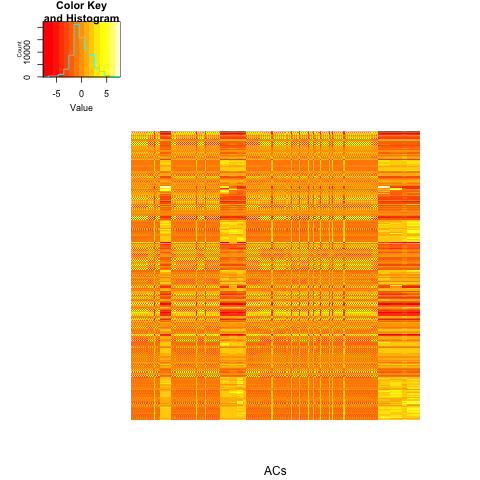
\includegraphics[width=0.3\textwidth]{../figure/HACH_plot.png}}
\caption{Heatmap of Dissimilarity measure for all networks}
\label{fig:table}    
\end{figure}


\begin{figure}[H]
\captionsetup{format=plain}
\centering
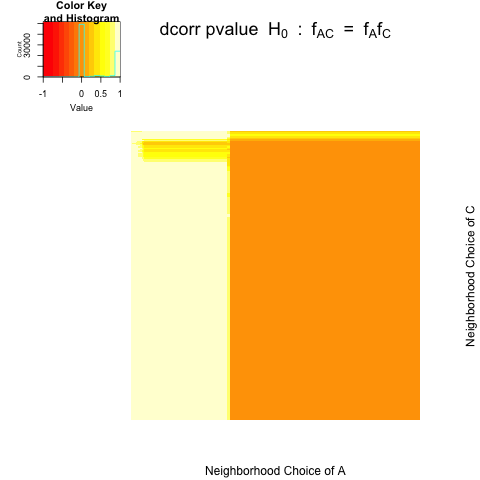
\includegraphics[width=0.4\textwidth]{../figure/P_A_C.png}
\caption{Local p-value matrix $A$ vs C}
\label{fig:PAC}
\end{figure} 

Figure \ref{fig:PAC} shows that p-values are largely dependent on neighboring choice of $A$ rather than that of $C$. It implies that the local p-values using a small number of neighbors in a neuronal network generally significant than those using a large number of neighbors, and their differences are larger than comparing the choice of distance matrix of cell types, $C$. 




%%%%%%%%%%%%%%%%%%%%%%%%%%%%%%%%%%%%%%%%%%%%%%%%%%%%%%%%%%%%%%%%%%%%%%%%%%
\newpage
Instead of using dissimilarity matrix for neuronal network $A$, Euclidean distance of $A^\prime$ is used to test the following hypothesis : 

\begin{center}\textbf{Goal : Test $H_{0} : f_{A^\prime C} = f_{A^\prime}f_{C}$}
\end{center}  

\begin{figure}[H]
\captionsetup{format=plain}
\subfigure[$A^\prime$]{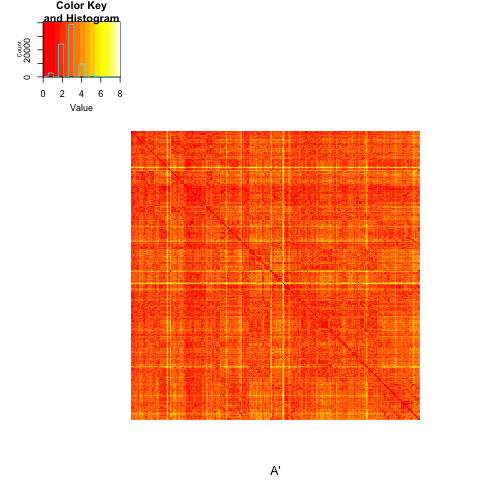
\includegraphics[width=0.3\textwidth]{../figure/A2_plot.png}}
\subfigure[$C$]{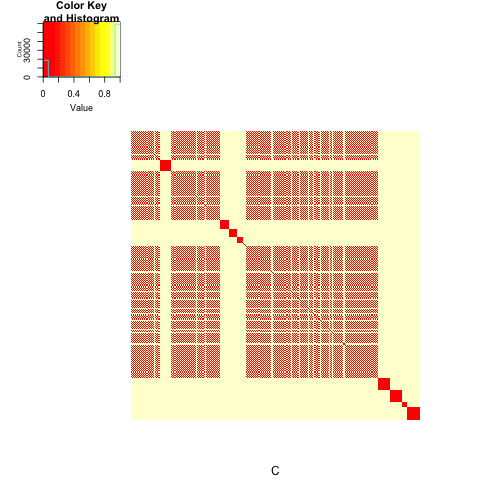
\includegraphics[width=0.3\textwidth]{../figure/C_plot.png}}
\subfigure[$A^\prime \cdot C$]{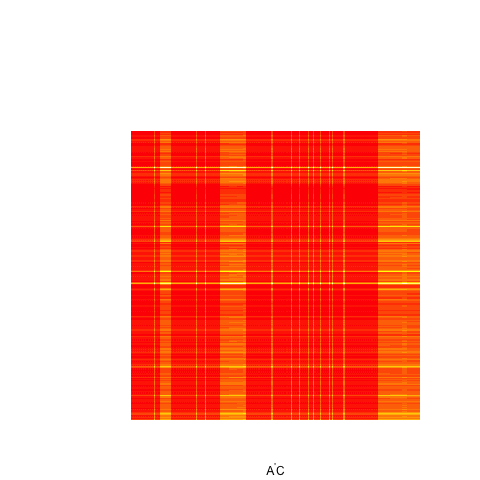
\includegraphics[width=0.3\textwidth]{../figure/A2C_plot.png}}
\subfigure[$\widetilde{A^\prime}$]{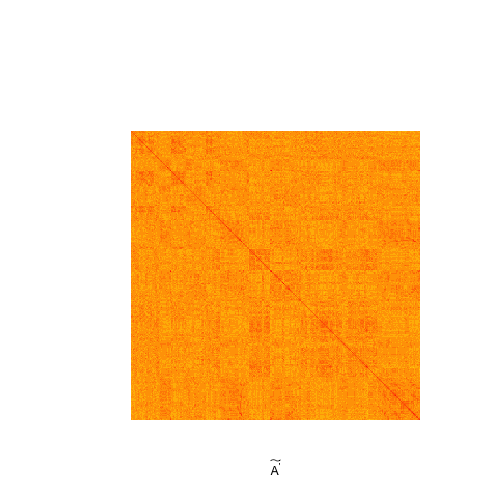
\includegraphics[width=0.3\textwidth]{../figure/HA2H.png}}
\subfigure[$\widetilde{C}$]{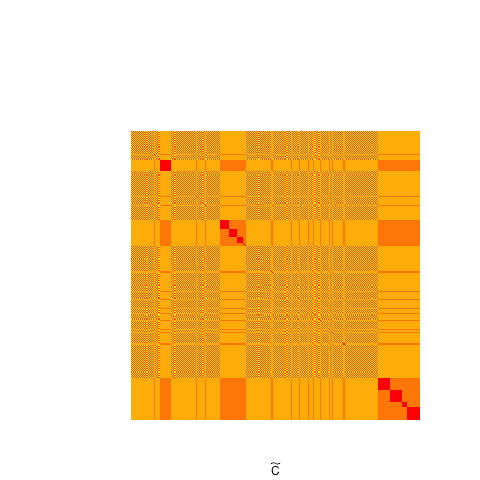
\includegraphics[width=0.3\textwidth]{../figure/HCH_plot.png}}
\subfigure[$\widetilde{A^\prime C}$]{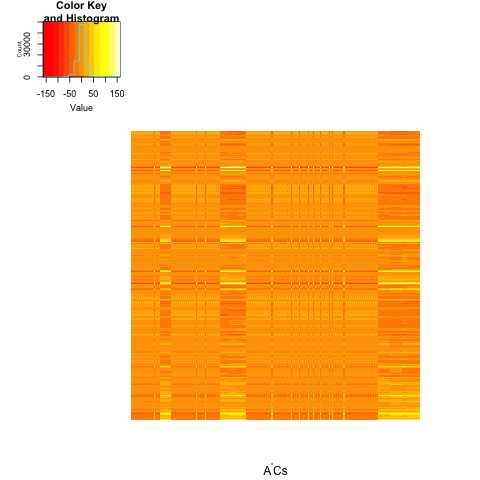
\includegraphics[width=0.3\textwidth]{../figure/HA2CH_plot.png}}
\caption{Heatmap of geodesic distance for all networks}
\label{fig:table}    
\end{figure}


\begin{figure}[H]
\captionsetup{format=plain}
\centering
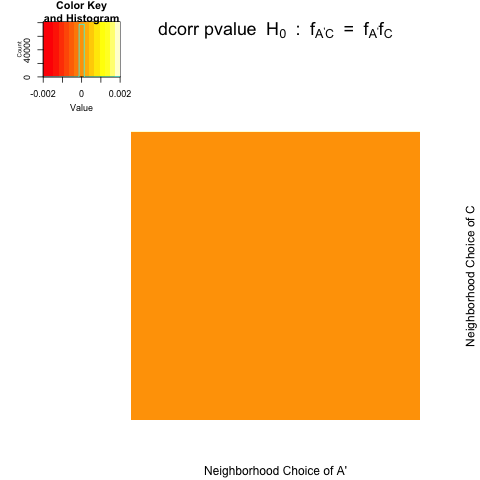
\includegraphics[width=0.4\textwidth]{../figure/P_A2_C.png}
\caption{Local p-value matrix $A^\prime$ vs C}
\label{fig:PA2C}
\end{figure} 

Compared to Figure \ref{PAC} where we used a dissimilarity matrix (modified adjacency matrix), Figure \ref{PA2C} illustrates significant p-values all over the local tests. 



%%%%%%%%%%%%%%%%%%%%%%%%%%%%%%%%%%%%%%%%%%%%%%%%%%%%%%%%%%%%%%%%%%%%%%%
\newpage
\section{Neuronal Network vs. Cell Direction}

Let's consider two categories in cell - "R"ight and "L"eft. Because 90 out of 279 nodes do not have information whether they are right or left, We can only consider an induced subnetwork comprised of 189 nodes. Let $A_{s}$ be a dissimilarity matrix of sub-network and $A^\prime_{s}$ be a geodesic distance matrix of subnetwork. Note that $A_{s}$ can be defined as a sub-matrix of $A,$ but how to define $A^\prime_{s}$ can be flexible - depending on whether you take account 90 nodes in calculating geodesic distance or not. I assume that a full network of 279 nodes well reflects all the connectivity, so include other 90 nodes in possible paths. Thus, $A^\prime_{s}$ can be also defined as a sub-matrix of $A^\prime.$
  
Let $D$ be a distance matrix of cell direction - Right or Left. 

\begin{center}\textbf{Goal : Test $H_{0} : f_{A_{s}D} = f_{A_{s}}f_{D}$}
\end{center}  


\begin{figure}[H]
\captionsetup{format=plain}
\subfigure[$A_{s}$]{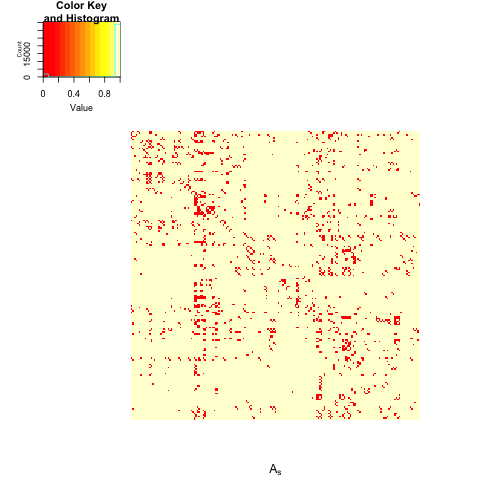
\includegraphics[width=0.3\textwidth]{../figure/As_plot.png}}
\subfigure[$D$]{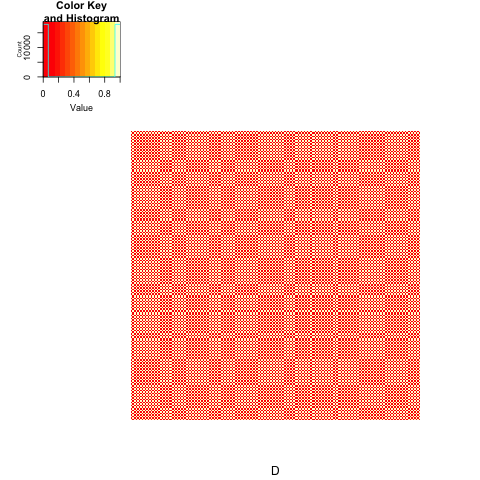
\includegraphics[width=0.3\textwidth]{../figure/D_plot.png}}
\subfigure[$A_{s} \cdot D$]{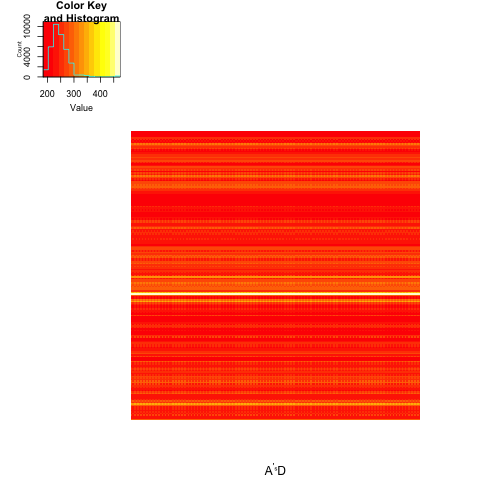
\includegraphics[width=0.3\textwidth]{../figure/AsD_plot.png}}
\subfigure[$\widetilde{A_{s}}$]{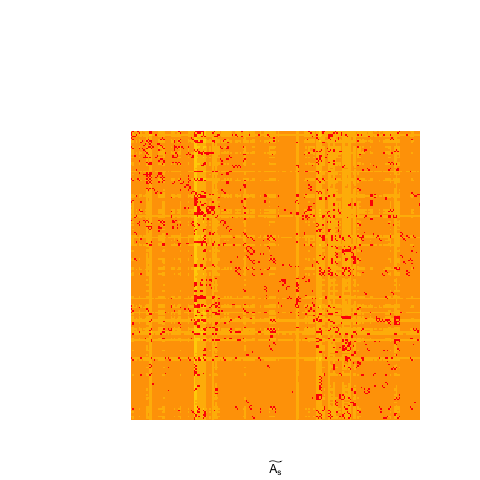
\includegraphics[width=0.3\textwidth]{../figure/HAsH_plot.png}}
\subfigure[$\widetilde{D}$]{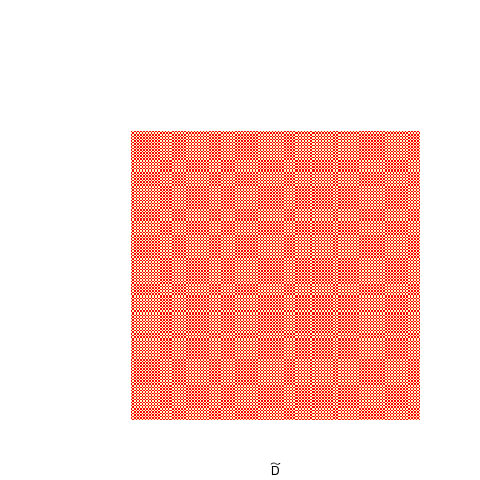
\includegraphics[width=0.3\textwidth]{../figure/HDH_plot.png}}
\subfigure[$\widetilde{A_{s} \cdot D}$]{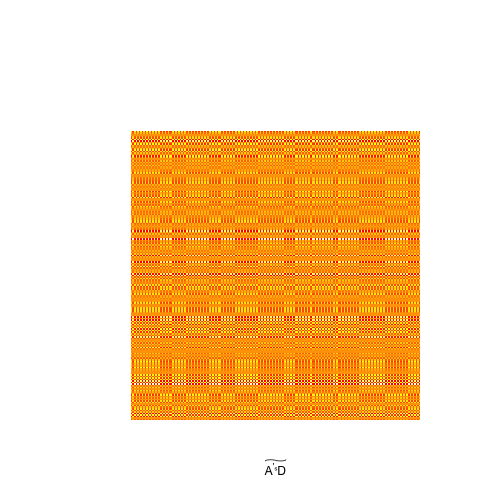
\includegraphics[width=0.3\textwidth]{../figure/HAsDH.png}}
\caption{Heatmap of Dissimilarity measure for subnetworks}
\label{fig:table}    
\end{figure}
 
 
\begin{figure}[H]
\captionsetup{format=plain}
\centering
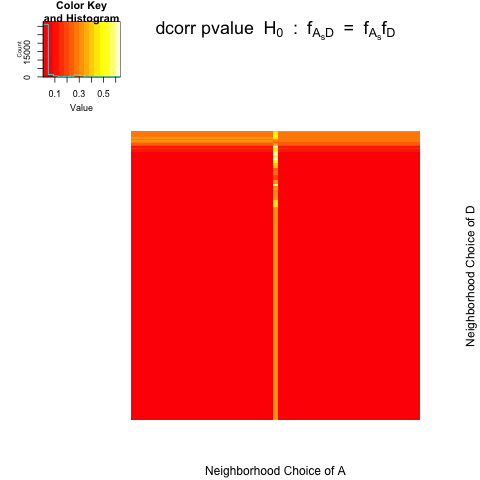
\includegraphics[width=0.4\textwidth]{../figure/P_A_D.png}
\caption{Local p-value matrix $A_{s}$ vs D}
\label{fig:PAD}
\end{figure} 

Interestingly, Figure \ref{fig:PAD} shows that using a certain range of neighbors in $A$, p-values are higher than (still could be significant at $\alpha = 0.05$, though) the other choices; while including more neighbors yields less p-values in the choice of distance $D$.  
 
 
 
\begin{figure}[H]
\captionsetup{format=plain}
\subfigure[$A^\prime_{s}$]{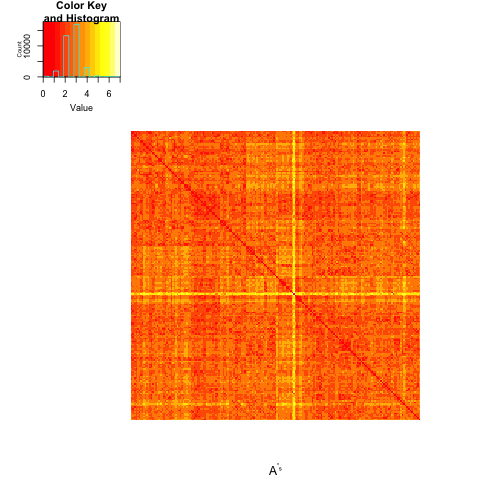
\includegraphics[width=0.3\textwidth]{../figure/A2s_plot.png}}
\subfigure[D]{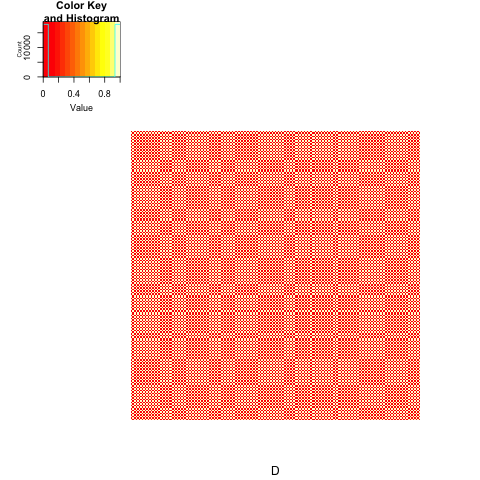
\includegraphics[width=0.3\textwidth]{../figure/D_plot.png}}
\subfigure[$A^\prime_{s} \cdot D$]{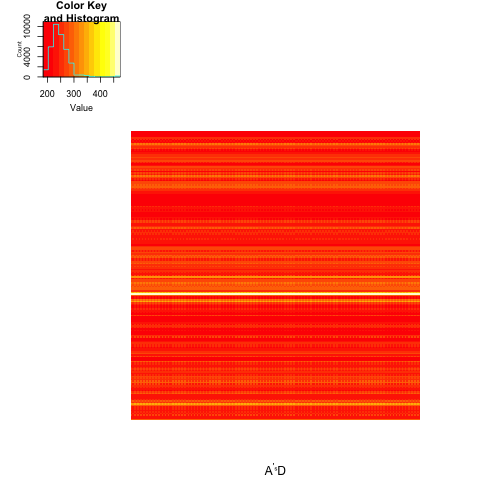
\includegraphics[width=0.3\textwidth]{../figure/AsD_plot.png}}
\subfigure[$\widetilde{A^\prime_{s}}$]{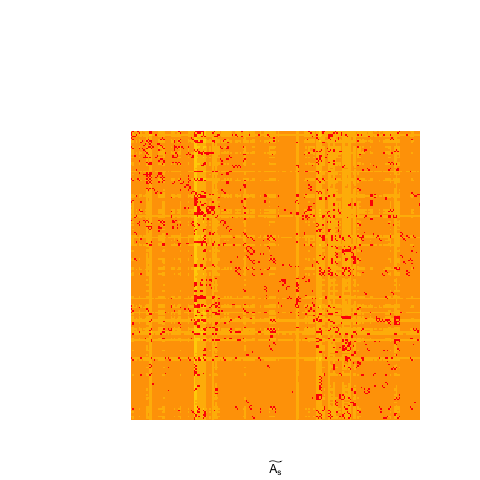
\includegraphics[width=0.3\textwidth]{../figure/HAsH_plot.png}}
\subfigure[$\widetilde{D}$]{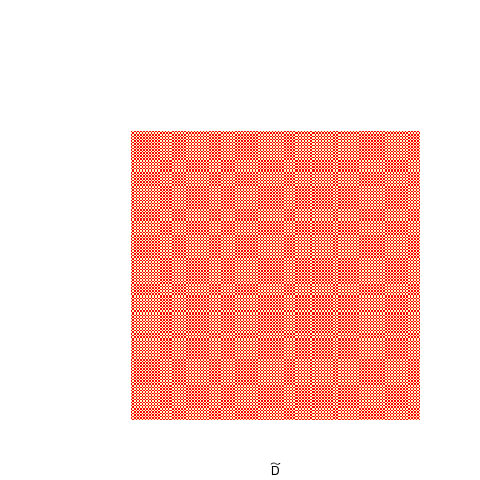
\includegraphics[width=0.3\textwidth]{../figure/HDH_plot.png}}
\subfigure[$\widetilde{A^\prime_{s} \cdot D}$]{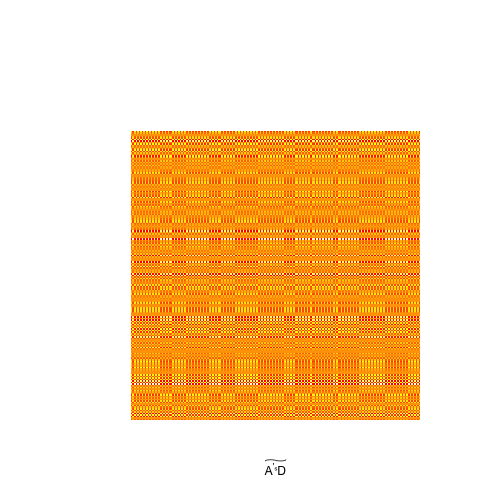
\includegraphics[width=0.3\textwidth]{../figure/HAsDH.png}}
\caption{Heatmap of Geodesic Distance for subnetworks}
\label{fig:table}    
\end{figure} 
 
 
\begin{figure}[H]
\captionsetup{format=plain}
\centering
\includegraphics[width=0.4\textwidth]{../figure/P_A2_D.png}
\caption{Local p-value matrix $A^\prime_{s}$ vs D}
\label{fig:PAD}
\end{figure} 

 
 
 
\end{document}

